\documentclass{beamer}
\usepackage{beamerthemeshadow}
\usepackage{verbatim}

\usepackage{lastpage}
\usepackage{xcolor}
\usepackage{pgf}
\usepackage{colortbl}
\usepackage{hyperref}
\usepackage{multirow}

\usepackage{siunitx}
\sisetup{input-symbols=(), group-digits  = false} 

\newcommand{\bi}{\begin{itemize}}
\newcommand{\ei}{\end{itemize}}
\newcommand{\be}{\begin{enumerate}}
\newcommand{\ee}{\end{enumerate}}
\newcommand{\bd}{\begin{description}}
\newcommand{\ed}{\end{description}}
\newcommand{\prbf}[1]{\textbf{#1}}
\newcommand{\prit}[1]{\textit{#1}}
\newcommand{\beq}{\begin{equation}}
\newcommand{\eeq}{\end{equation}}
\newcommand{\bdm}{\begin{displaymath}}
\newcommand{\edm}{\end{displaymath}}

\newcommand{\ft}[1]{
  \frametitle{\begin{tabular}{p{4.2in}r} \textcolor{white}{#1} & \small{\insertframenumber / \inserttotalframenumber} \end{tabular}}
  \setbeamercovered{transparent=18}
}

\newcommand{\eft}[1]{
  \frametitle{\begin{tabular}{p{4in}r} \textcolor{white}{#1} & \small{\hyperlink{f:questions}{\beamergotobutton{GO BACK}}} \end{tabular}}
  \setbeamercovered{transparent=18}
}

\newcommand{\stepinv}{\setbeamercovered{invisible}}
\newcommand{\stopinv}{\setbeamercovered{transparent=18}}
\newcommand{\uncoverinv}[1]
{
  \setbeamercovered{invisible}
  \uncover<+->{#1}
  \setbeamercovered{transparent=18}
}
\newcommand{\ans}[1]{\textcolor{blue}{#1}}
\newcommand{\ansinv}[1]
{
  \setbeamercovered{invisible}
  \uncover<+->{\textcolor{blue}{#1}}
  \setbeamercovered{transparent=18}
}
\newcommand{\setinv}{\setbeamercovered{invisible}}
\newcommand{\setvis}{\setbeamercovered{transparent=18}}
\newcommand{\centerpic}[2]
{
  \begin{center}
  \includegraphics[#1]{#2}
  \end{center}
}
\newcommand{\h}[1]{\hat{#1}}
\newcommand{\ds}{\displaystyle}

\definecolor{light}{rgb}{1.0,0.7,0.7}
\definecolor{BrickRed}{rgb}{0.8,0.1,0.1}
%\definecolor{light}{rgb}{1.0,0.5,0.5}
\newcommand{\hl}[1]{\only<#1>{\cellcolor{light}}}

\definecolor{mycolor}{rgb}{0.6,0.0,0.0}
\usecolortheme[named=mycolor]{structure}

\title[Fiscal Policy Uncertainty and Macroeconomic Consequences]{Identifying Fiscal Policy Uncertainty and Its Macroeconomic Consequences}
\author[James Murray, University of Wisconsin - La Crosse]
{
James Murray\\
Department of Economics\\
University of Wisconsin - La Crosse
}
\date{November 25, 2013}

\begin{document}

\frame{\titlepage \setcounter{framenumber}{0}}

\frame
{
  \ft{Purpose}
  \begin{block}{Quantify Fiscal Policy Uncertainty}
    \bi
    \item Time-varying volatility of a DSGE fiscal shock:\\
      ~~~Fern\'andez-Villiverde et. al. (2011), Born and Pfeifer (2011).
    \item Index based on newspaper headlines and other real world stuff:\\
      ~~~Baker et. al. (2013)
    \ei
  \end{block}

  \begin{block}{Present Paper}
      \bi
      \item Market participants behave like empirical economists - they estimate fiscal policy rules.
      \item Least-squares learning re: fiscal policy behavior
      \item Eg: Early sections of Fern\'andez-Villiverde et. al. (2011), Born and Pfeifer (2011).
      \item Forecast uncertainty:  Fiscal policy uncertainty should be related to the variance of forecasts.
      \ei
  \end{block}
}

\frame
{
  \ft{Fiscal Uncertainty Consequences for Macroeconomy}
  \begin{block}{Fiscal Policy Variables}
    \begin{columns}
    \begin{column}{0.4\textwidth}
    \be
    \item Government Spending
    \item Tax Revenue
    \item Net Transfers
    \item Government Debt
    \ee
    \end{column}

    \begin{column}{0.5\textwidth}
        \textit{Least-squares learning for each.}\\
\ \\
        \textit{Construct an uncertainty measure for each.}
    \end{column}
    \end{columns}
  \end{block}

  \begin{block}{Impact on Macroeconomy}
  Incorporate measures of fiscal uncertainty in a VAR including:
    \be
    \item Consumption
    \item Investment
    \item Real GDP
    \item Unemployment
    \ee  
  \end{block}
}

\frame
{
  \ft{Motivation}
  \begin{block}{Historical Economic and Political Crises}
  \bi
  \item Financial crisis and historic economic downturn.
  \item Large monetary and fiscal policy responses, fiscal policy multiplier debate is still active.
  \item U.S. Government Debt to GDP reaching historical levels.
  \item Simultaneous calls from left and right calling for opposing fiscal responses.
  \ei
  \end{block}

  \begin{block}{Ben Bernanke - July 2012 Monetary Policy Report to Congress}
    \textit{``The most effective way that the Congress could help to support the economy right now would be to work to address the nation's fiscal challenges....  \textbf{\textit{Doing so earlier rather than later would help reduce uncertainty and boost household and business confidence.}}''}
  \end{block}
}

\frame
{
  \ft{Literature}
  \begin{block}{Time-varying Fiscal Volatility}
  \bi
  \item Fern\'andez-Villiverde et. al. (2011a): Fiscal policy uncertainty is stagflationary
  \item Born and Pfeifer (2011): 
    \bi
    \item Significant evidence for time-varying volatility in fiscal shocks.
    \item Not a significant driver for business cycles.
    \ei
  \item Johannsen (2012): Matters more at ZLB.
  \ei
  \end{block}

  \begin{block}{Macroeconomic Impact of Volatility}
    \bi
    \item Bloom (2009, \textit{Econometrica})
    \item Bloom et. al. (2012)
    \item Fern\'andez-Villiverde et. al. (2011b, \textit{AER})
    \ei
  \end{block}

  \begin{block}{Fiscal Uncertainty}
  Baker (2013): Reduces economic activity
  \end{block}
}


\frame
{
  \ft{Spoiler}
  \begin{block}{Fiscal Uncertainty Reduces Economic Activity}
  \bi
  \item Investment is adversely affected by,
    \bi
    \item Government spending uncertainty
    \item Tax uncertainty
    \ei
  \item Consumption and real GDP adversely affected by,
    \bi
    \item Tax uncertainty
    \item Government debt uncertainty
    \item These findings are less robust than above to VAR specification.
    \ei
  \ei
  \end{block}

  \begin{block}{But it may boost the labor market!}
  Unemployment decreases with transfers uncertainty.
  \end{block}

}

\frame
{
  \ft{Constant Gain Learning}
  \begin{block}{Constant gain learning mechanism}
    \bi
    \item Every period, run a least-squares regression for each fiscal policy variable, using data from previous periods.
    \item Weighted least squares - more recent observations have more weight.
    \item Regression forecast serves as expectation.
    \item Root (weighted) mean squared error serves as \textit{fiscal policy uncertainty}.
    \ei
  \end{block}

 \begin{block}{Ideal situations for constant gain learning}
    \bi
    \item Precedence of structural changes
    \item No a-priori knowledge on menu or evolution of structural changes and probability distributions
    \item Forecasting rule, but no knowledge of parameter values, or the structure of the whole economy.
    \ei
  \end{block}

}

\frame
{
  \ft{Fiscal Policy Regressions}
  \begin{block}{Empirical Model for Fiscal Policy Behavior}
  Each fiscal policy variable ($f_{i,t}$) responds to:
  \bi
  \item Lag of all fiscal policy variables ($f_{t-1}$).
  \item Above includes lag of government debt ($b_{t-1}$).
  \item Macro outcomes: real GDP ($y_t$), consumption ($c_t$), investment ($I_t$), and unemployment ($u_t$).
  \item All quantities real, per capita, ratio of past real GDP.
  \ei
  \end{block}

  \begin{block}{Four regressions}
  \textbf{Fiscal policy variables:} $f_{t} = [g_t~ r_t~ n_t~ b_t]$ \\ 
  Govt Spending ($g_t$), Tax Revenue ($r_t$),\\
  Net Transfers ($n_t$), Government Debt / GDP ($b_t$) \\ [0.5pc]

  \textbf{Regression equation:}\\
  $f_{i,t} = \alpha_{t,0} + \alpha_{t,f}' f_{t-1} + \alpha_{t,y} y_{t} + \alpha_{t,c} c_t + \alpha_{I,t} I_t + \alpha_{t,u} u_{t} + \epsilon_t$
  \end{block}
}

\frame
{
  \ft{Least-Squares Learning}
  \begin{scriptsize}
  \begin{block}{OLS Regression}
    \bdm \hat{\alpha}_t = \left(\sum_{\tau=0}^{t} X_{\tau} X_{\tau}' \right)^{-1} \left(\sum_{\tau=0}^{t} X_{\tau}' f_{i,\tau} \right) \edm
    \bi
    \item $X_{\tau} = [1~ f'_{\tau-1}~ y_{\tau}~ c_\tau~ I_\tau~ u_{\tau}]'$ is vector of regressors.
    \item Predicted fiscal policy action: $E_t^* f_{i,t} = X_t' \hat{\alpha}_t$
    \item Unexplained policy: $\hat{\epsilon}_t = f_{i,t} - X_t' \hat{\alpha}_t$
    \ei
  \end{block}

  \begin{block}{Recursive Formulation}
  The OLS regression coefficients can be rewritten as:
    \bdm \begin{array}{c}
      \hat{\alpha}_{i,t} = \alpha_{i,t-1} + \gamma_{t} R_t^{-1} X_t (f_t - X_t' \hat{\alpha}_t) \\ [1pc] 
      R_t = R_{t-1} + \gamma_{t} (X_t X_t' - R_{t-1}),
    \end{array}\edm
  where $\gamma_{t} = 1/t$ is the \textbf{learning gain}.
  \end{block}
  \end{scriptsize}
}

\frame
{
  \ft{Constant-Gain Learning}
  \begin{footnotesize}
  \begin{block}{Recursive Formulation}
    \bdm \begin{array}{c}
      \hat{\alpha}_{i,t} = \alpha_{i,t-1} + \gamma R_t^{-1} X_t (f_{i,t} - X_t' \hat{\alpha}_{i,t}) \\ [1pc] 
      R_t = R_{t-1} + \gamma (X_t X_t' - R_{t-1}),
    \end{array}\edm
    \bi
    \item Learning gain, $\gamma \in (0,1)$, is constant, equal to the weight assigned to most recent observation.
    \item Typical estimates for $\gamma \sim 0.02$ (Milani (2008), Slobodyan and Wouters (2008)).
    \ei
  \end{block}

  \begin{block}{Standard Formulation}
    \bdm \hat{\alpha}_{i,t} = \left( (1-\gamma)  \sum_{\tau=1}^{t} \gamma^{\tau} X_{t-\tau} X_{t-\tau}' \right)^{-1}  \left( (1-\gamma)  \sum_{\tau=1}^{t} \gamma^{\tau} X_{t-\tau}  f_{i,t-\tau} \right). \edm
    Weight on $t-\tau$ observation declines geometrically with $\tau$: $\omega_\tau = (1-\gamma) \gamma^{\tau}$.
  \end{block}
  \end{footnotesize}
}

\frame
{
  \ft{Instrumental Variable (IV) Regression} 
  \begin{block}{Endogeneity Problem}
  \bi 
  \item Macro outcomes (real GDP, consumption, investment, and unemployment) are likely endogenous.
  \item Maybe market participants account for that.
  \item Use instruments: lags of macro outcomes and fiscal variables
  \ei
  \end{block}

  \begin{block}{Instrumental Variables Notation}
  \bi
  \item Let $W_{t} = [y_{t}~ c_t~ I_{t}~ u_{t}]'$ denote the possibly endogenous regressors in $X_{t}$,
  \item Let $V_{t} = [1~ f'_{t-1}]'$ denote the remaining exogenous regressors
  \item Then, $X_{t} = [V_t'~ W_{t}']'$.
  \item Let $S_t = [W'_{t-1}~ W'_{t-2}~ f'_{t-2} ]$ denote vector of instruments.
  \item Let $Z_t = [V'_t~ S'_t]'$ denote vector Stage 1 IV regressors.
  \ei
  \end{block}
}

\frame
{
  \ft{Two-Stage IV Least-Squares Learning}
  \begin{block}{Stage 1: Endogenous macro variable on instruments + exogenous}
    $W_{i,t} = Z_{t}' \beta_i + \upsilon_{i,t}$.\\[0.3pc]
    $\hat{\beta}_{i,t} = \hat{\beta}_{i,t-1} + \gamma \left(R_t^{S1}\right)^{-1} Z_{t-1} \left(W_{i,t-1} - Z_{t-1}'\hat{\beta}_{i,t-1}\right)$ \\ [0.3pc]
    $R_t^{S1} = R_{t-1}^{S1} + \gamma \left(Z_{t-1} Z_{t-1}' - R_{t-1}^{S1}\right)$ 
  \end{block}

  \begin{block}{Save Stage 1 Predicted Values}
  $\hat{W}_{i,t} = Z_{t}' \hat{\beta}_{i,t},~~~  \hat{X}_t = [V_t'~ \hat{W}_t']'$
  \end{block}

  \begin{block}{Stage 2: Constant Gain Learning with IV}
    $\hat{\alpha}_{i,t}^{IV} = \hat{\alpha}_{i,t-1}^{IV} + \gamma \left(R_t^{S2}\right)^{-1} \hat{x}_{t-1} \left(f_{i,t-1} - \hat{X}_{t-1}'\hat{\alpha}_{i,t-1}\right)$ \\ [0.3pc]
    $R_t^{S2} = R_{t-1}^{S2} + \gamma \left(\hat{X}_{t-1} \hat{X}_{t-1}' - R_{t-1}^{S2}\right)$. 
  \end{block}
}

\frame
{
  \ft{Fiscal Policy Uncertainty}
  \bi
  \item Unexplained fiscal policy:\\
    \bdm \epsilon_{i,t} = f_{i,t} - \hat{\alpha}_{i,t}^{IV'} X_t \edm

\ \\

  \item Forecast uncertainty $\sim$ Root (weighted) mean squared error:\\
    \bdm m_{i,t}^{IV} = \sqrt{ (1-\gamma) \ds \sum_{\tau=1}^{t} \gamma^{\tau} \epsilon_{i,t}^2} \edm
  \ei
}

\frame
{
  \ft{Forecast Uncertainty vs. Time-Varying Volatility}
  \begin{block}{Time-varying Volatility}
  \bi
  \item Eg: Fern\'andez-Villiverde et. al. (2011), Born and Pfeifer (2011), Johannsen (2012), etc.
  \item Can separate causal effects of fiscal shocks from i.i.d. innovations to variance.
  \item Possibly unrealistic set of knowledge and perceptions.
  \item Is fiscal policy uncertainty exogenous?
  \ei
  \end{block}

  \begin{block}{Forecast Uncertainty}
  \bi
  \item Agents are learning fiscal policy processes.
  \item Constant gain learning: accounts for structural change possibility.
  \item Fiscal shocks can move expectations away from true model.
  \item Time-varying uncertainty need not depend on time-varying volatility.
  \ei
   
  \end{block}
}

\frame
{
  \ft{Fiscal Policy - Actual and Predicted}
  \begin{tabular}{cc}
    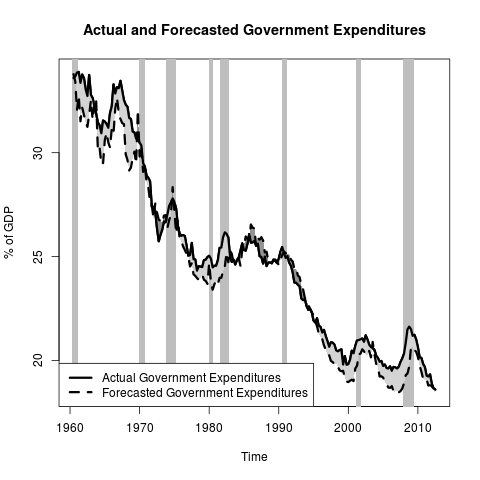
\includegraphics[width=0.45\textwidth, height=0.45\textheight]{uncertainty_pics/pred_gov.png} & 
    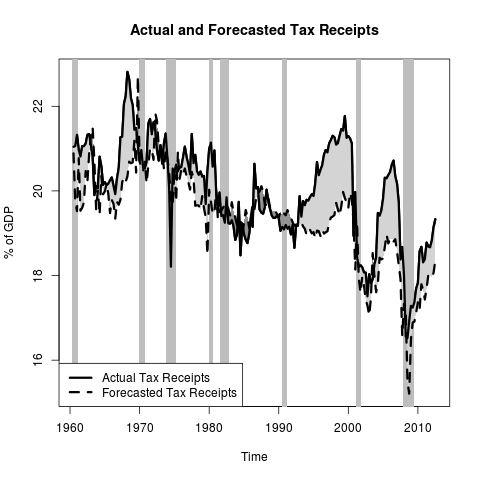
\includegraphics[width=0.45\textwidth, height=0.45\textheight]{uncertainty_pics/pred_tax.png} \\ 
    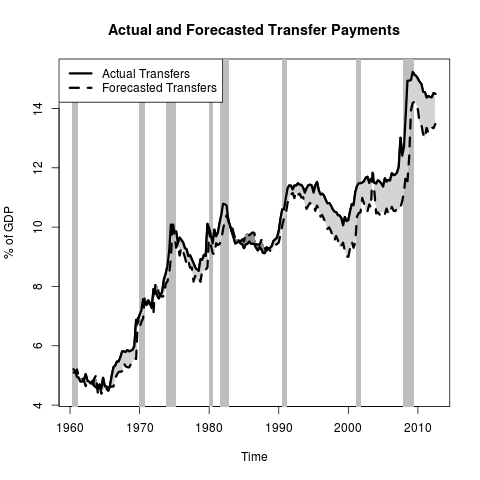
\includegraphics[width=0.45\textwidth, height=0.45\textheight]{uncertainty_pics/pred_transfers.png} & 
    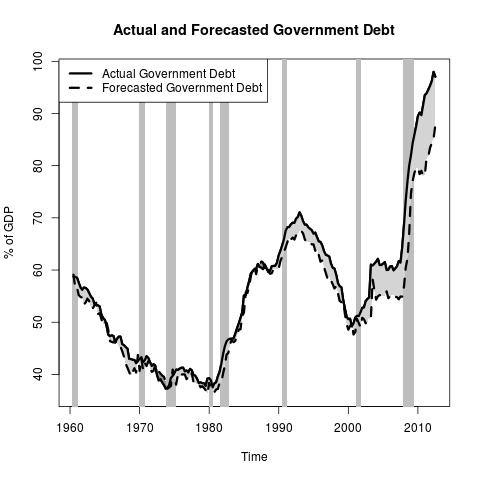
\includegraphics[width=0.45\textwidth, height=0.45\textheight]{uncertainty_pics/pred_debt.png} 
  \end{tabular}
}

\frame
{
  \ft{Fiscal Policy - Forecast Error}
  \begin{tabular}{cc}
    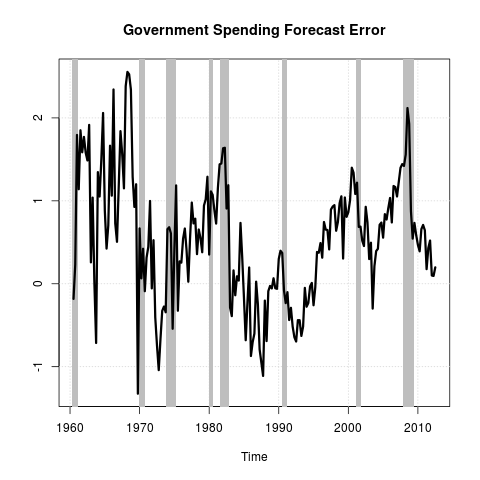
\includegraphics[width=0.45\textwidth, height=0.45\textheight]{uncertainty_pics/fe_gov.png} & 
    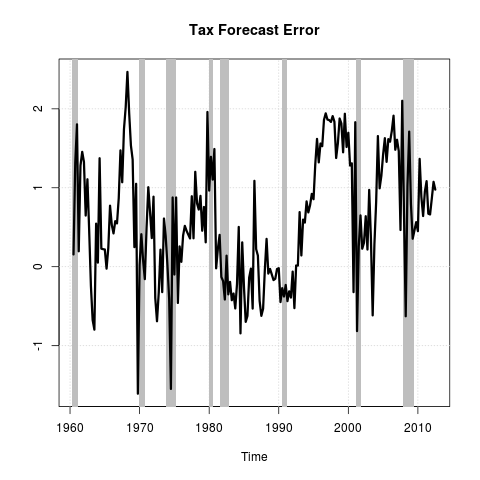
\includegraphics[width=0.45\textwidth, height=0.45\textheight]{uncertainty_pics/fe_tax.png} \\ 
    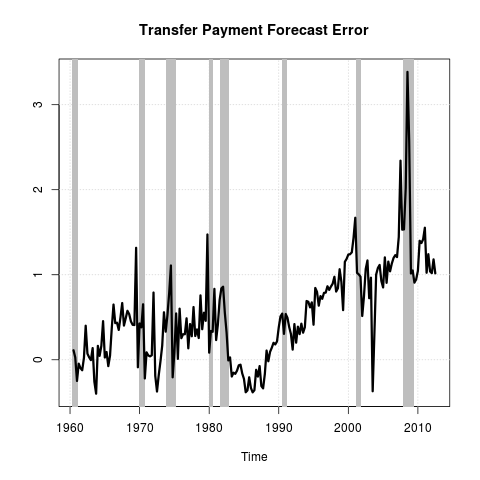
\includegraphics[width=0.45\textwidth, height=0.45\textheight]{uncertainty_pics/fe_transfers.png} & 
    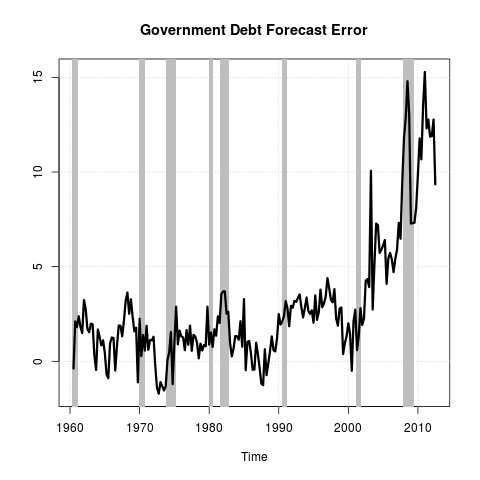
\includegraphics[width=0.45\textwidth, height=0.45\textheight]{uncertainty_pics/fe_debt.png} 
  \end{tabular}
}

\frame
{
  \ft{Fiscal Policy Uncertainty}
  \begin{tabular}{cc}
    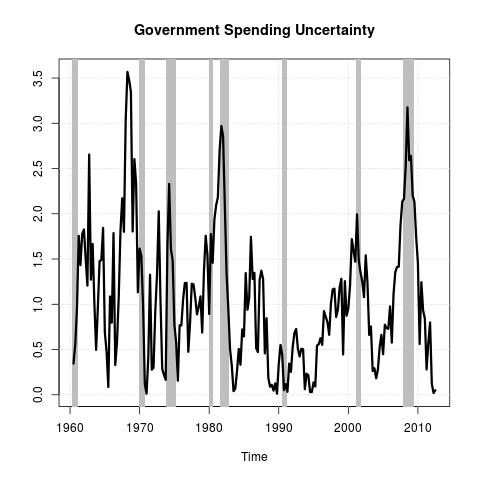
\includegraphics[width=0.45\textwidth, height=0.45\textheight]{uncertainty_pics/fpu_gov.png} & 
    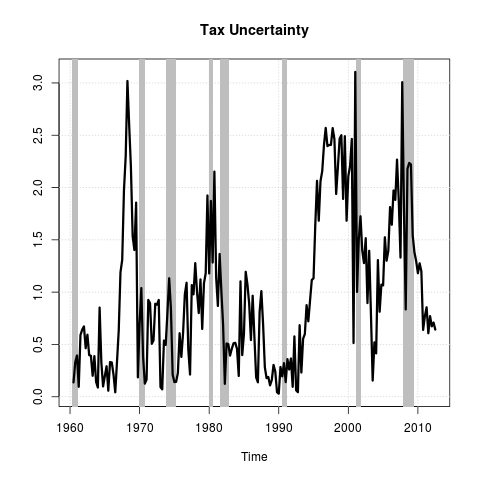
\includegraphics[width=0.45\textwidth, height=0.45\textheight]{uncertainty_pics/fpu_tax.png} \\ 
    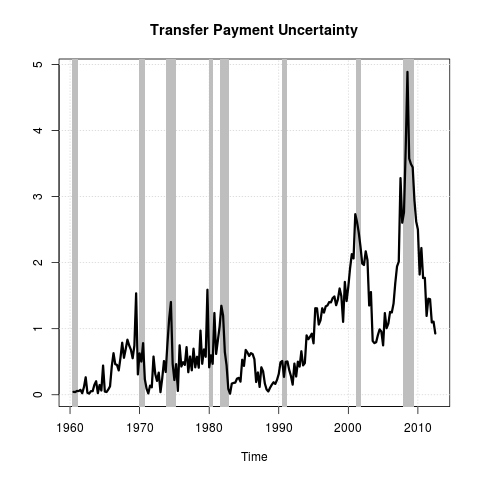
\includegraphics[width=0.45\textwidth, height=0.45\textheight]{uncertainty_pics/fpu_transfers.png} & 
    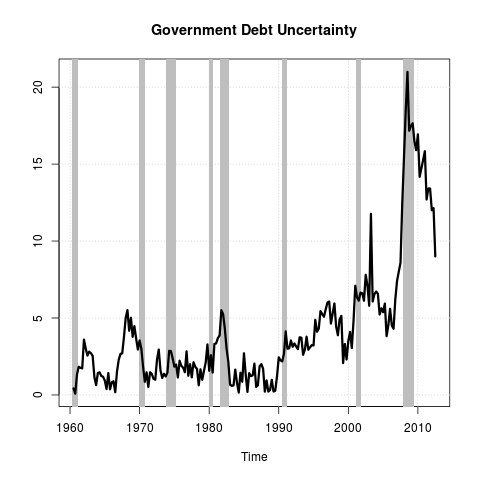
\includegraphics[width=0.45\textwidth, height=0.45\textheight]{uncertainty_pics/fpu_debt.png} 
  \end{tabular}
}

\frame
{
  \ft{Casual Observations}
  \bi
  \item Uncertainty concerning transfers and debt reached unprecedented levels during Great Recession.
    \bi
    \item Transfers uncertainty: Nearly 5\% of GDP
    \item Government debt uncertainty: Exceeded 20\% of GDP
    \ei
  \item Tax and government spending uncertainty reached near highs of about 3\% of GDP
  \item Uncertainty seems to run up for several years preceding recessions:
    \bi
    \item Early 1980s, 2001, 2007.
    \item Not the rule though (eg: declines prior to 1970s, not much action prior to 1991)
    \ei
  \ei
}

\frame
{
  \ft{Macroeconomic Consequences}
  \bi
  \item Answer this with a reduced form vector autoregression in:
    \be
    \item Real GDP
    \item Consumption
    \item Investment
    \item Unemployment
    \ee
  \item Augment explanatory variables with fiscal policy uncertainty variables (first lag)
  \item Consider VAR lag lengths: 1, 2, and 4.
  \item Consider learning gain parameters: $\gamma=0.01,~ 0.02,~0.03$.
  \ei
}

\frame[t]
{
  \ft{VAR Results: Real GDP}
\begin{scriptsize}
\begin{center}
\textbf{Dependent Variable: Real GDP}\\
\textbf{Learning Gain: $\gamma=0.01$}\\
\end{center}

\begin{center}
\begin{tabular}{l|p{4pc}p{4pc}p{4pc}}\hline
 & \multicolumn{1}{c}{1 Lag} & \multicolumn{1}{c}{2 Lags} & \multicolumn{1}{c}{4 Lags} \\ \hline 
\multirow{13}{*}{\begin{tabular}{l} Expenditures Uncertainty \hl{2} \\ (Standard Error)$^2$ \hl{2} \\ [0.25pc] Tax Uncertainty \\ (Standard Error) \\ [0.25pc] Transfers Uncertainty \\ (Standard Error) \\ [0.25pc] Debt Uncertainty \hl{3} \\ (Standard Error) \hl{3} \\ [0.25pc] Joint F-test \hl{4} \\ [0.25pc] Adjusted R-square \\ AIC \\ BIC \end{tabular}}
& \multirow{13}{*}{\begin{tabular}{S[table-format=3.3]}
-0.191$^{*}$ \hl{2} \\
(0.116) \hl{2} \\ [0.25pc]
-0.050$^{}$ \\
(0.208) \\ [0.25pc]
0.270$^{}$ \\
(0.191) \\ [0.25pc]
-0.077$^{**}$ \hl{3} \\
(0.039) \hl{3} \\ [0.25pc]
\multicolumn{1}{S[table-format=3.1]}{4.1$^{***}$ \hl{4}} \\ [0.25pc]
\multicolumn{1}{S[table-format=1.3]}{0.240} \\ \multicolumn{1}{S[table-format=3.1]}{478.9} \\ \multicolumn{1}{S[table-format=3.1]}{532.3} \end{tabular}}
& \multirow{13}{*}{\begin{tabular}{S[table-format=3.3]}
-0.091$^{}$ \hl{2} \\
(0.113) \hl{2} \\ [0.25pc]
-0.170$^{}$ \\
(0.216) \\ [0.25pc]
0.410$^{}$ \\
(0.141) \\ [0.25pc]
-0.071$^{**}$ \hl{3} \\
(0.040) \hl{3} \\ [0.25pc]
\multicolumn{1}{S[table-format=3.1]}{2.7$^{**}$ \hl{4}} \\ [0.25pc]
\multicolumn{1}{S[table-format=1.3]}{0.346} \\ \multicolumn{1}{S[table-format=3.1]}{456.7} \\ \multicolumn{1}{S[table-format=3.1]}{543.5} \end{tabular}}
& \multirow{13}{*}{\begin{tabular}{S[table-format=3.3]}
-0.234$^{**}$ \hl{2} \\
(0.121) \hl{2} \\ [0.25pc]
-0.226$^{}$ \\
(0.219) \\ [0.25pc]
0.465$^{}$ \\
(0.112) \\ [0.25pc]
-0.031$^{}$ \hl{3} \\
(0.046) \hl{3} \\ [0.25pc]
\multicolumn{1}{S[table-format=3.1]}{2.8$^{**}$ \hl{4}} \\ [0.25pc]
\multicolumn{1}{S[table-format=1.3]}{0.409} \\ \multicolumn{1}{S[table-format=3.1]}{451.6} \\ \multicolumn{1}{S[table-format=3.1]}{605.1} \end{tabular}}
\\  & & &   \\  & & & \\  & & & \\  & & &  \\  & & & \\  & & & \\ & & & \\ & & & \\ & & & \\  & & & \\  & & & \\  & & & \\  & & & \\ \hline 
\end{tabular}
\end{center}
\end{scriptsize}

\only<1>{ \ \\ \ \\}
\only<2>{\textcolor{BrickRed}{\textbf{Some evidence expenditures uncertainty decreases real GDP.}}}
\only<3>{\textcolor{BrickRed}{\textbf{Debt uncertainty decreases real GDP.}}}
\only<4>{\textcolor{BrickRed}{\textbf{Fiscal policy uncertainty matters one way or another.}}}

}

\frame[t]
{
  \ft{VAR Results: Consumption}
\begin{scriptsize}
\begin{center}
\textbf{Dependent Variable: Consumption}\\
\textbf{Learning Gain: $\gamma=0.01$}\\
\end{center}

\begin{center}
\begin{tabular}{l|p{4pc}p{4pc}p{4pc}}\hline
 & \multicolumn{1}{c}{1 Lag} & \multicolumn{1}{c}{2 Lags} & \multicolumn{1}{c}{4 Lags} \\ \hline 
\multirow{13}{*}{\begin{tabular}{l} Expenditures Uncertainty \\ (Standard Error)$^2$ \\ [0.25pc] Tax Uncertainty \\ (Standard Error) \\ [0.25pc] Transfers Uncertainty \\ (Standard Error) \\ [0.25pc] Debt Uncertainty \hl{2} \\ (Standard Error) \hl{2} \\ [0.25pc] Joint F-test \hl{3} \\ [0.25pc] Adjusted R-square \\ AIC \\ BIC \end{tabular}}
& \multirow{13}{*}{\begin{tabular}{S[table-format=3.3]}
0.073$^{}$ \\
(0.072) \\ [0.25pc]
-0.080$^{}$ \\
(0.083) \\ [0.25pc]
0.070$^{}$ \\
(0.089) \\ [0.25pc]
-0.052$^{***}$ \hl{2} \\
(0.020) \hl{2} \\ [0.25pc]
\multicolumn{1}{S[table-format=3.1]}{3.8$^{***}$ \hl{3} } \\ [0.25pc]
\multicolumn{1}{S[table-format=1.3]}{0.980} \\ \multicolumn{1}{S[table-format=3.1]}{179.4} \\ \multicolumn{1}{S[table-format=3.1]}{232.8} \end{tabular}}
& \multirow{13}{*}{\begin{tabular}{S[table-format=3.3]}
0.065$^{}$ \\
(0.067) \\ [0.25pc]
-0.179$^{*}$ \\
(0.119) \\ [0.25pc]
0.123$^{}$ \\
(0.081) \\ [0.25pc]
-0.035$^{*}$ \hl{2}  \\
(0.026) \hl{2}  \\ [0.25pc]
\multicolumn{1}{S[table-format=3.1]}{2.6$^{**}$ \hl{3} } \\ [0.25pc]
\multicolumn{1}{S[table-format=1.3]}{0.980} \\ \multicolumn{1}{S[table-format=3.1]}{187.7} \\ \multicolumn{1}{S[table-format=3.1]}{274.5} \end{tabular}}
& \multirow{13}{*}{\begin{tabular}{S[table-format=3.3]}
0.010$^{}$ \\
(0.058) \\ [0.25pc]
-0.065$^{}$ \\
(0.129) \\ [0.25pc]
0.089$^{}$ \\
(0.081) \\ [0.25pc]
-0.026$^{}$ \hl{2}  \\
(0.026) \hl{2}  \\ [0.25pc]
\multicolumn{1}{S[table-format=3.1]}{0.8$^{}$ \hl{3} }   \\ [0.25pc]
\multicolumn{1}{S[table-format=1.3]}{0.981} \\ \multicolumn{1}{S[table-format=3.1]}{198.2} \\ \multicolumn{1}{S[table-format=3.1]}{351.7} \end{tabular}}
\\  & & &   \\  & & & \\  & & & \\  & & &  \\  & & & \\  & & & \\ & & & \\ & & & \\ & & & \\  & & & \\  & & & \\  & & & \\  & & & \\ \hline 
\end{tabular}
\end{center}
\end{scriptsize}

\only<1>{ \ \\ \ \\}
\only<2>{\textcolor{BrickRed}{\textbf{Some evidence that debt uncertainty decreases consumption.}}}
\only<3>{\textcolor{BrickRed}{\textbf{Fiscal policy uncertainty likely influences consumption.}}}

}

\frame[t]
{
  \ft{VAR Results: Investment}
\begin{scriptsize}
\begin{center}
\textbf{Dependent Variable: Investment}\\
\textbf{Learning Gain: $\gamma=0.01$}\\
\end{center}

\begin{center}
\begin{tabular}{l|p{4pc}p{4pc}p{4pc}}\hline
 & \multicolumn{1}{c}{1 Lag} & \multicolumn{1}{c}{2 Lags} & \multicolumn{1}{c}{4 Lags} \\ \hline 
\multirow{13}{*}{\begin{tabular}{l} Expenditures Uncertainty \hl{2} \\ (Standard Error)$^2$ \hl{2} \\ [0.25pc] Tax Uncertainty \hl{3} \\ (Standard Error) \hl{3} \\ [0.25pc] Transfers Uncertainty \\ (Standard Error) \\ [0.25pc] Debt Uncertainty \\ (Standard Error) \\ [0.25pc] Joint F-test \hl{4} \\ [0.25pc] Adjusted R-square \\ AIC \\ BIC \end{tabular}}
& \multirow{13}{*}{\begin{tabular}{S[table-format=3.3]}
-0.248$^{***}$ \hl{2} \\
(0.064) \hl{2} \\ [0.25pc]
-0.223$^{*}$ \hl{3} \\
(0.163) \hl{3} \\ [0.25pc]
0.319$^{}$ \\
(0.115) \\ [0.25pc]
0.008$^{}$ \\
(0.035) \\ [0.25pc]
\multicolumn{1}{S[table-format=3.1]}{5.3$^{***}$ \hl{4}} \\ [0.25pc]
\multicolumn{1}{S[table-format=1.3]}{0.943} \\ \multicolumn{1}{S[table-format=3.1]}{304.0} \\ \multicolumn{1}{S[table-format=3.1]}{357.4} \end{tabular}}
& \multirow{13}{*}{\begin{tabular}{S[table-format=3.3]}
-0.152$^{***}$ \hl{2} \\
(0.058) \hl{2} \\ [0.25pc]
-0.209$^{*}$ \hl{3} \\
(0.141) \hl{3} \\ [0.25pc]
0.339$^{}$ \\
(0.103) \\ [0.25pc]
0.012$^{}$ \\
(0.021) \\ [0.25pc]
\multicolumn{1}{S[table-format=3.1]}{3.0$^{**}$ \hl{4} } \\ [0.25pc]
\multicolumn{1}{S[table-format=1.3]}{0.958} \\ \multicolumn{1}{S[table-format=3.1]}{249.7} \\ \multicolumn{1}{S[table-format=3.1]}{336.4} \end{tabular}}
& \multirow{13}{*}{\begin{tabular}{S[table-format=3.3]}
-0.216$^{***}$ \hl{2} \\
(0.063) \hl{2} \\ [0.25pc]
-0.296$^{***}$ \hl{3} \\
(0.126) \hl{3} \\ [0.25pc]
0.391$^{}$ \\
(0.092) \\ [0.25pc]
0.035$^{}$ \\
(0.020) \\ [0.25pc]
\multicolumn{1}{S[table-format=3.1]}{4.2$^{***}$ \hl{4}} \\ [0.25pc]
\multicolumn{1}{S[table-format=1.3]}{0.962} \\ \multicolumn{1}{S[table-format=3.1]}{243.4} \\ \multicolumn{1}{S[table-format=3.1]}{396.9} \end{tabular}}
\\  & & &   \\  & & & \\  & & & \\  & & &  \\  & & & \\  & & & \\ & & & \\ & & & \\ & & & \\  & & & \\  & & & \\  & & & \\  & & & \\ \hline 
\end{tabular}
\end{center}
\end{scriptsize}

\only<1>{ \ \\ \ \\}
\only<2>{\textcolor{BrickRed}{\textbf{Expenditures uncertainty decreases investment.}}}
\only<3>{\textcolor{BrickRed}{\textbf{Tax uncertainty likely decreases investment.}}}
\only<4>{\textcolor{BrickRed}{\textbf{Fiscal policy uncertainty likely influences investment.}}}


}

\frame[t]
{
  \ft{VAR Results: Unemployment}
\begin{scriptsize}
\begin{center}
\textbf{Dependent Variable: Unemployment}\\
\textbf{Learning Gain: $\gamma=0.01$}\\
\end{center}

\begin{center}
\begin{tabular}{l|p{4pc}p{4pc}p{4pc}}\hline
 & \multicolumn{1}{c}{1 Lag} & \multicolumn{1}{c}{2 Lags} & \multicolumn{1}{c}{4 Lags} \\ \hline 
\multirow{13}{*}{\begin{tabular}{l} Expenditures Uncertainty \\ (Standard Error)$^2$ \\ [0.25pc] Tax Uncertainty \\ (Standard Error) \\ [0.25pc] Transfers Uncertainty\hl{2} \\ (Standard Error) \hl{2} \\ [0.25pc] Debt Uncertainty \\ (Standard Error) \\ [0.25pc] Joint F-test \hl{3} \\ [0.25pc] Adjusted R-square \\ AIC \\ BIC \end{tabular}}
& \multirow{13}{*}{\begin{tabular}{S[table-format=3.3]}
0.049$^{}$ \\
(0.035) \\ [0.25pc]
0.185$^{}$ \\
(0.099) \\ [0.25pc]
-0.107$^{**}$ \hl{2} \\
(0.048) \hl{2}\\ [0.25pc]
0.008$^{}$ \\
(0.023) \\ [0.25pc]
\multicolumn{1}{S[table-format=3.1]}{7.6$^{***}$ \hl{3}} \\ [0.25pc]
\multicolumn{1}{S[table-format=1.3]}{0.977} \\ \multicolumn{1}{S[table-format=3.1]}{23.8} \\ \multicolumn{1}{S[table-format=3.1]}{77.2} \end{tabular}}
& \multirow{13}{*}{\begin{tabular}{S[table-format=3.3]}
-0.002$^{}$ \\
(0.031) \\ [0.25pc]
0.115$^{}$ \\
(0.088) \\ [0.25pc]
-0.115$^{**}$ \hl{2} \\
(0.052) \hl{2} \\ [0.25pc]
0.016$^{}$ \\
(0.015) \\ [0.25pc]
\multicolumn{1}{S[table-format=3.1]}{2.6$^{**}$ \hl{3} } \\ [0.25pc]
\multicolumn{1}{S[table-format=1.3]}{0.982} \\ \multicolumn{1}{S[table-format=3.1]}{-22.1} \\ \multicolumn{1}{S[table-format=3.1]}{64.7} \end{tabular}}
& \multirow{13}{*}{\begin{tabular}{S[table-format=3.3]}
0.018$^{}$ \\
(0.030) \\ [0.25pc]
0.119$^{}$ \\
(0.079) \\ [0.25pc]
-0.108$^{***}$ \hl{2} \\
(0.045) \hl{2} \\ [0.25pc]
0.013$^{}$ \\
(0.015) \\ [0.25pc]
\multicolumn{1}{S[table-format=3.1]}{2.1$^{*}$ \hl{3}} \\ [0.25pc]
\multicolumn{1}{S[table-format=1.3]}{0.982} \\ \multicolumn{1}{S[table-format=3.1]}{1.2} \\ \multicolumn{1}{S[table-format=3.1]}{154.7} \end{tabular}}
\\  & & &   \\  & & & \\  & & & \\  & & &  \\  & & & \\  & & & \\ & & & \\ & & & \\ & & & \\  & & & \\  & & & \\  & & & \\  & & & \\ \hline 
\end{tabular}
\end{center}
\end{scriptsize}

\only<1>{ \ \\ \ \\}
\only<2>{\textcolor{BrickRed}{\textbf{Transfers uncertainty $decreases$ unemployment.}}}
\only<3>{\textcolor{BrickRed}{\textbf{Fiscal policy uncertainty likely influences unemployment.}}}
}

\frame
{
  \ft{Summary of Findings}
  \begin{block}{Fiscal Uncertainty Reduces Economic Activity}
  \bi
  \item Investment is adversely affected by,
    \bi
    \item Government spending uncertainty
    \item Tax uncertainty
    \ei
  \item Consumption and real GDP adversely affected by,
    \bi
    \item Tax uncertainty
    \item Government debt uncertainty
    \item These findings are less robust than above to VAR specification.
    \ei
  \ei
  \end{block}

  \begin{block}{But it may boost the labor market!}
  Unemployment decreases with transfers uncertainty.
  \end{block}
}

\end{document}

